\chapter{IoT Voting System Implementation}
\section{Hardware Setup}
The experimental setup comprises the following components:
\begin{itemize}
    \item \textbf{Tallier Node:} Sony Vaio E Series laptop (Intel Core i5-2450M, 8 GB DDR3 RAM) running Antix Linux 23.1, serving three critical roles:
    \begin{itemize}
        \item Wi-Fi Access Point (using hostapd v2.9)
        \item MQTT Broker (using Eclipse Mosquitto v2.0.20)
        \item Election Tallier
    \end{itemize}
    
    \item \textbf{Guardian Nodes:} 2× NodeMCU ESP32 boards (ESP32-WROOM-32 modules) with:
    \begin{itemize}
        \item 240 MHz dual-core Xtensa LX6 CPU
        \item 520 KB SRAM, 4 MB flash
        \item Integrated 802.11 b/g/n Wi-Fi
    \end{itemize}
\end{itemize}

\section{Election Setup}
The Guardian nodes are responsible for distributing trust in the encryption and decryption processess managed by the Tallier. Their responsibilities are divided into two main phases: the key generation ceremony, and the decryption process.

\subsection{Cryptographic constants} \label{sec:constants}
Before implementing the ElectionGuard specification, it is essential to establish the mathematical constants for the cryptographic operations. ElectionGuard specifies standard values for the primes (p) and (q) and a generator (g) \cite[21]{eg-spec}. The standard baseline parameters include:
\begin{itemize}
    \item A 4096-bit prime (p) \cite[22]{eg-spec}
    \item A 4096-bit generator (g) \cite[23]{eg-spec}
    \item A 256-bit prime (q) \cite[21]{eg-spec}
\end{itemize}

For this experiment, we will use reduced parameters that offer better performance at a lower security level \cite[23]{eg-spec}. The reduced parameters are defined as  
\begin{itemize}
    \item A 3072-bit prime (p) \cite[36]{eg-spec}
    \item A 3072-bit generator (g) \cite[36-37]{eg-spec}
    \item A 256-bit prime (q) \cite[36]{eg-spec}
\end{itemize}

\subsection{Pre-Election Key Generation}
The pre-election phase involves administrative tasks necessary to configure the election, including the key generation ceremony.

\begin{figure}
    \centering
    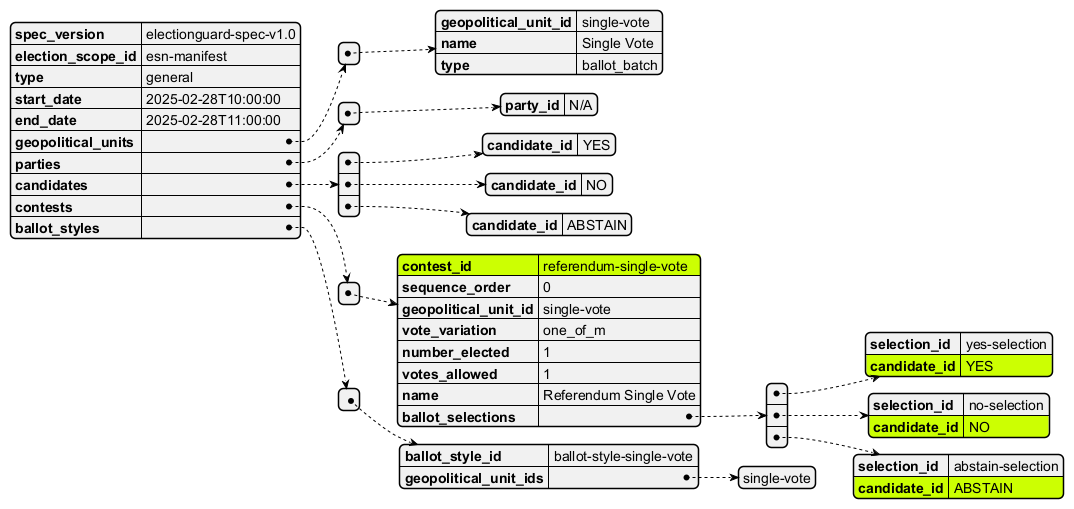
\includegraphics[width=\textwidth]{abbildungen/Diagramme/manifest.png}
    \caption{Visualisation of the JSON Election Manifest}
    \label{Fig:manifest}
\end{figure}

The tallier node defines the election manifest, sets the cryptographic constants according to the reduced baseline parameters (as discussed in \ref{sec:constants}), and sets the quorum size. Given that only two Guardian nodes are available for this experiment the quorum size is set to two. Figure \ref{Fig:manifest} shows a visualisation of the election manifest used in this election. The election is limited to a simple YES/NO/ABSTAIN referendum. The Tallier collaborates with the Guardians to generate a joint key used to encrypt the ballots in the next election phase.

\begin{figure}
    \centering
    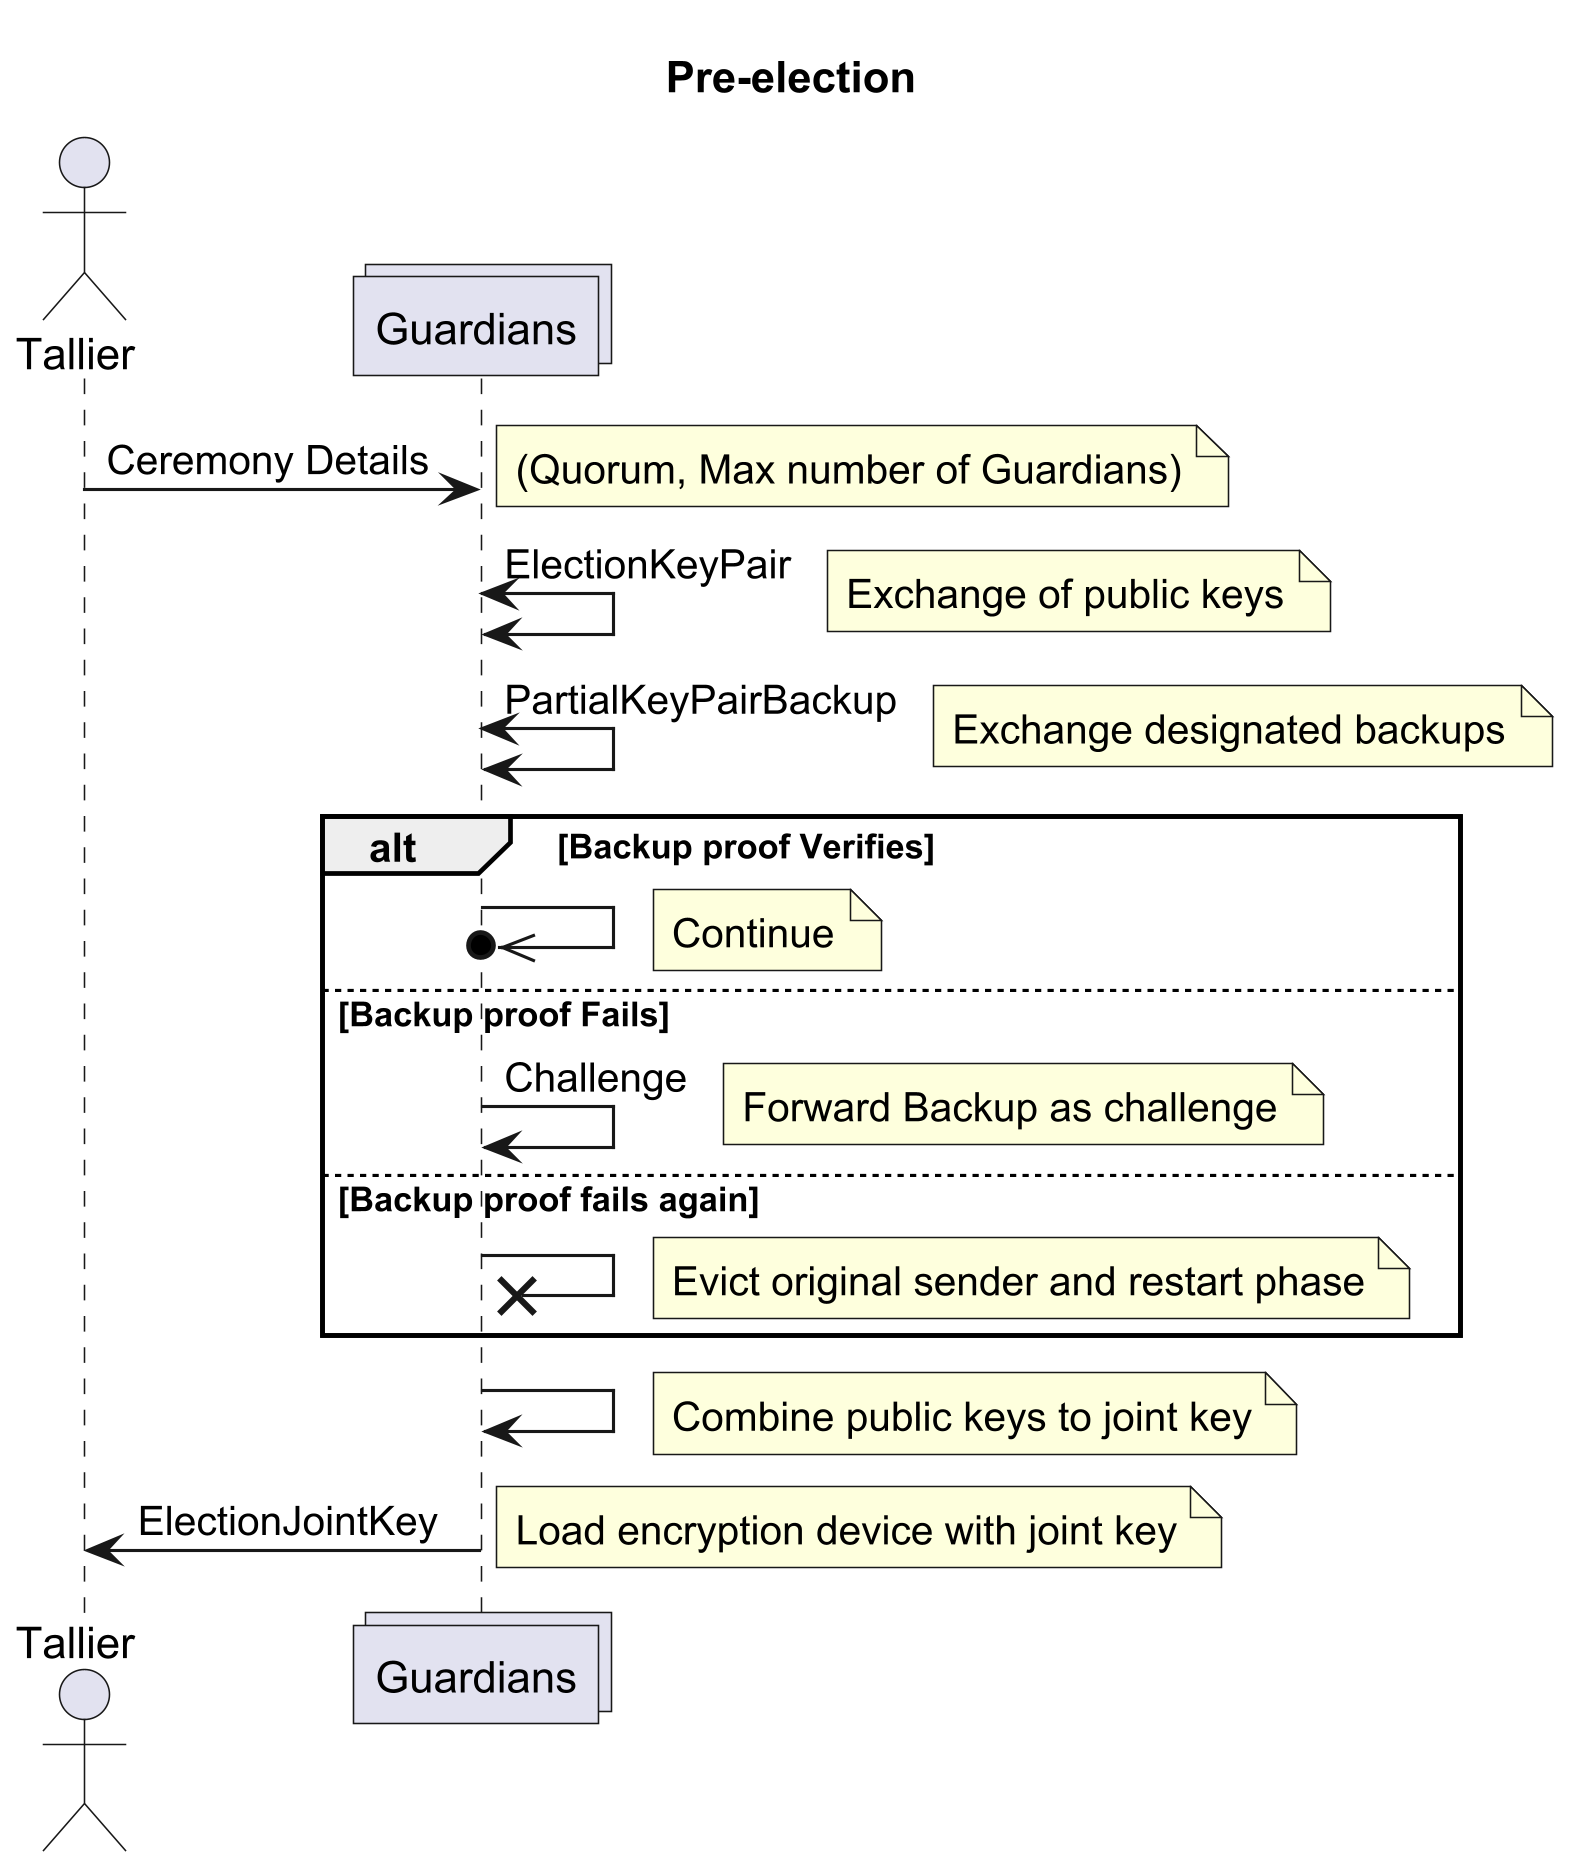
\includegraphics[width=0.8\textwidth]{abbildungen/Diagramme/communication-seq0.png}
    \caption{Communication Sequence in the Pre-election phase}
    \label{Fig:comm-pre}
\end{figure}

Figure \ref{Fig:comm-pre} illustrates the communication sequence involved in this phase. The Tallier sends the ceremony details required for the key generation ceremony to the Guardians. The quorum size influences how each Guardian generates their ElectionKeyPair. After generating their ElectionKeyPair and stripping the secret key for transmission, the Guardians exchange their ElectionKeyPairs. Each Guardian generates a designatted backup for each ElectionKeyPair received, which is then sent back to the sending Guardian. Each backup contains a proof that must be verified by the receiver. The challenge mechanism and eviction mechanism for failed verifications are not implemented in this experiment. This verification process for a challenge or a backup is identical. Once all backups successfully verify, the ElectionKeyPairs are combined into a joint key.

\subsection{Intra-Election Ballot Encryption}
During this election, the Tallier simulates the voting process by generating random ballots and encrypting them using the joint key established in the previous phase. The ballots are cast and processed as detailed in Appendix \ref{lst:intra-election}.

\subsection{Post-Election Decryption of Tallies}
In the post-election phase, all encrypted ballots from the previous phase are homomorphically aggregated to produce an encrypted tally. This encrypted tally is send to the Guardians for decryption. Each guardian uses their private key to generate a decryption share, which is essentialy a partial decryption. The Tallier then combines all decryption shares into a decrypted tally. Figure \ref{Fig:comm-post} illustrates the communication involved in this phase. The decryption of spoiled ballots is optional and not implemented in this experiment. The decryption process of the spoiled ballots mirrors that of the encrypted tallly. The case of missing Guardians is also not addressed in this experiment. Compensating for missing decryptions functions similarly to the generation of the decryption share. The publication of the election artifacts is also not implemented. Publishing the election artifacts is not implemented,  the interaction between the Guardians and the Tallier requires inherent verification due to the proofs involved.

\begin{figure}
    \centering
    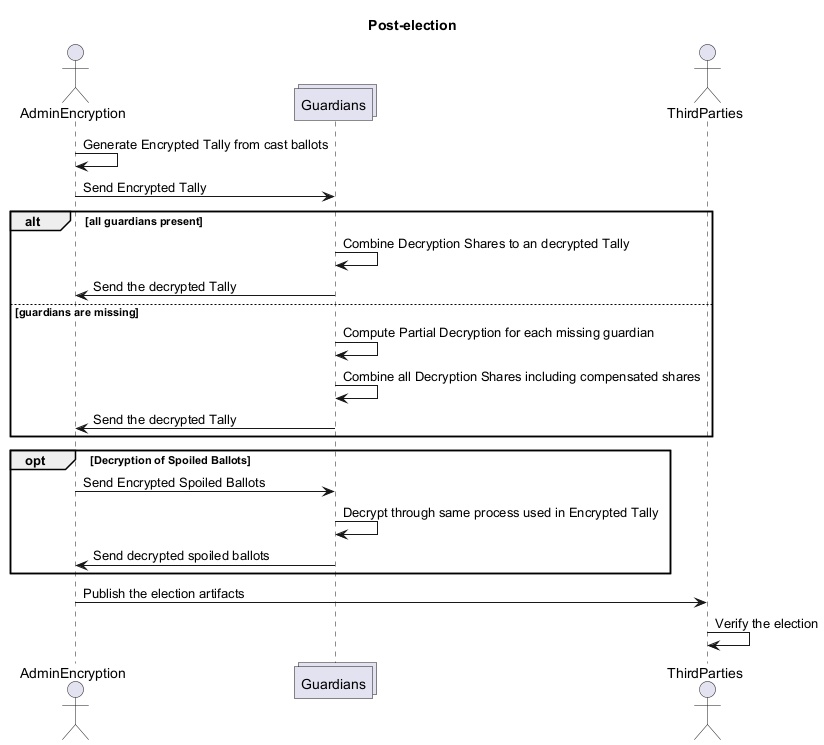
\includegraphics[width=\textwidth]{abbildungen/Diagramme/communication-seq2.png}
    \caption{Communication Sequence in the Post-election phase}
    \label{Fig:comm-post}
\end{figure}

\section{Comparison of ElectionGuard Implementations}
Due to the open-source nature of ElectionGuard, various community ports exist, such as a Java port \cite{eg-docs}. However, this discussion focuses solely on the official ports from Microsoft. There are 2 ElectionGuard libraries implementing the ElectionGuard 1.0 specification: a Python reference implementation and a C++ reference implementation. The Python implementation encompasses the entire suite of functionality and processes necessary to implement \ac{E2E} verifiable election as part of a voting system \cite{python-reference}. It is designed to be universal and portable, albeit less performant \cite{eg-docs}. In contrast, the C++ reference implementation focuses solely on the encryption components and is optimized for execution on low-powered devices \cite{cpp-reference}. 

\subsection{Python Reference}
Running the Python reference implementation on the ESP32 may be feasible through \textbf{MicroPython}, an implementation of Python 3.x targeted for microcontrollers and embedded systems. MicroPython adapts standard Python library functionalities to accommodate the limitations inherent of microcontrollers, such as restricted memory and processing speed \cite{micropython} \cite[234]{micropython-performance}. There are drawbacks to this approach, as essential modules, functions, and classes may be absent in MicroPython \cite{micropython}. Additionally, applications developed in MicroPython are prone to memory fragmentation and may experience issues with objects expending in size. \cite[234]{micropython-performance}. A comparative study of software-based SHA-256 computation for the ESP32 revealed that the performance of MicroPython was inferior to that of a C implementation \cite[237]{micropython-performance}. For instance, the C implementation outperformed the MicroPython implementation by 45\% \cite[237]{micropython-performance}.

The Electionguard Python is not designed to be performant, and compatibility issues may arise when using MicroPython, along with potential memory fragmentation problems. Due to these limitations, the Python reference implementation may not be the most suitable choice for the ESP32. However, it remains a valuable resource for understanding the ElectionGuard specification and can serve as a reference for developing a possible port. Our Tallier node, which has more computational resource compared to our Guardians, will run the Python reference implementation as a Python package for convenience.

\subsection{C++ Reference}
The ElectionGuard C++ reference implements focuses solely on the encryption library, omitting abstractions such as Guardians. This implementation is designed for execution on low-powered devices with Intel Atom-level processor performance in mind \cite{cpp-reference} \cite{eg-docs}. Porting the C++ library to an ESP32 should be feasible, as ESP-IDF supports C++ application development. Certain C++ features, such as exception handling, must be enabled in the project configuration beforehand. The ESP32 also supports C++ threads, which are implemented as wrappers around C pthreads, which in turn wrap around FreeRTOS tasks \cite{esp-prog}. 

Compared to the Python implementation, the C++ implementation incorporates optimisations to accelerate computations of certain modular exponentiations \cite{cpp-reference}. These optimisations come at a memory cost. The optimisation for modular exponentiation uses pre-computed tables to speed up calculations for certain exponentiations \cite{cpp-reference}. A modular exponentiation computes \(X^Y \mod P\). This optimization is possible because many of the exponentiations in ElectionGuard are performed with a fixed base, such as the generator (g). The pre-computed table contains certain powers of these bases, allowing the computation \(G^Y\) to be turned into a series of table lookups \cite[22-23]{eg-paper}.

To store the table, we must consider the capabilities of the ESP32. The ESP32 has 520 KB of volatile memory (SRAM) and 4 MB of non-volatile memory (in-package flash). The SRAM is divided into 320 KB of DRAM and 200 KB of IRAM. IRAM is used for instruction memory, while DRAM is used for data memory. The maximum statically allocated DRAM usage is 160 KB, the remaining 160 KB can only be allocated as heap memory \cite{esp32-ref}. 

\begin{lstlisting}[language=C++, caption={FixedBaseTable Definition}]
    typedef std::array<std::array<uint64_t[MAX_P_LEN], OrderBits>, TableLength> FixedBaseTable;
\end{lstlisting}

The lookup table (FixedBaseTable) is implemented and tuned to the following values. Any modifications to these parameters could affect the function's internal operations.
\begin{itemize}
    \item b= 256 (OrderBits)
    \item k = 8 (WindowSize)
    \item m = 32 (TableLength)
\end{itemize}

To estimate the memory requirements of the \textbf{FixedBaseTable}, we can calculate the total size in bytes as follows:
\begin{equation}
    \mathrm{FixedBaseTable Size} = \mathrm{sizeof(uint64\_t)} \times \mathrm{MAX\_P\_LEN} \times \mathrm{OrderBits} \times \mathrm{TableLength}
\end{equation}
Given that MAX\_P\_LEN is defined as 64 (4096-bit), we will calulate with 48 (3072-bit) since we are using the reduced baseline parameters. Substituting the values into the equation gives:
\begin{equation}
    \mathrm{FixedBaseTable Size} = 8 \times 48 \times 256 \times 32 =  3145728 \mathrm{ bytes} = 3 \mathrm{ MB}
\end{equation}

Consequently, the \textbf{FixedBaseTable} exceeds the volatile memory capacity of the ESP32. Although storing the table in the non-volatile memory might be feasible, it may require further optimizations because it must accommodate the bootloader and the application binary. Reducing the \textbf{WindowSize} would result in smaller tables and reduced memory usage, but it simultaneously increases the number of multiplications \cite[22]{eg-spec}. Given these memory requirements, it is evident that the C++ implementation would require further optimizations to be feasible on the ESP32. Therefore, we opt to implement a native C implementation based on the Python reference implementation.

\subsection{Implementation Strategy for ESP32}
ElectionGuard uses integer ElGamal cryptography within its specific cryptographic operations. The system performs four key operations on very large integer values: \textbf{modular exponentiation}, \textbf{modular multiplication}, \textbf{modular addition}, and \textbf{SHA-256} hash computation. 

To handle the large integer values involved in these operations, specialized libraries for large integers may be employed, or the operations can be developed from scratch \cite[21, 25-26]{eg-spec}. When developing these modular operations from the ground up, it is common for intermediate values to become excessively large. Techniques such as modular reduction are often necessary to ensure that values remain manageable \cite[21, 25-26]{eg-spec}. Consequently, employing fast libraries for modular arithmetic becomes crucial for achieving good performance \cite[22]{eg-paper}. The Python implementation uses the C-coded GnuMP library for large integer arithmetic, the C++ implementation uses HACL* a performant C implementation of a wide variety of cryptographic primitives \cite[22]{eg-paper} \cite{cpp-reference}. In ESP32 cryptographic primitives are implemented through a fork of the mbedTLS library. Optionally, a port of the WolfSSL library is also available \cite{esp32-ref}. The benefit of these two libraries over the other mentioned libraries is that these libraries include patches related to hardware routines for on-board cryptographic hardware acceleration \cite{esp32-ref} \cite[114]{wolfSSL-manual}. The ESP32 supports supports several cryptographic hardware acceleration capabilities including AES, SHA, RSA, and RNG as illustrated in the functional block diagram \ref{Fig:esp32-crypto}. These hardware accelerators significantly enhance operational speed and reduce software complexity for the aforementioned cryptographic primitives \cite[32]{esp32-series}. More details on the hardware acceleration capabilities of the ESP32 are provided in Section \ref{sec:hardware-acceleration}.

Figure \ref{Fig:software-components} detauls the ESP32 software stack
\begin{figure}
	\centering
	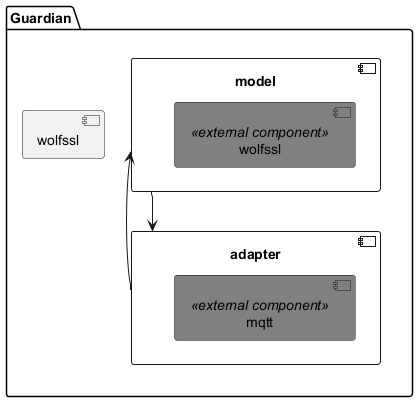
\includegraphics[scale=.5]{abbildungen/Diagramme/components.png}
	\caption{Software components for the Guardian Prototype}\label{Fig:software-components} 
\end{figure}

Figure \ref{Fig:software-components} depicts the software components used in the Guardian ESP32 port. The model component includes the business logic for the guardians operations. The adapter component implements the communication aspects. The adapter component calls the model component to perform guardian specific operations. The model component uses the wolfSSL library for cryptographic primitives. The wolfSSL component is overwritten using c pre-processor macros to reduce the binary size by removing unused features. Furthermore, the library is configured to run on the memory-restricted ESP32 by configuring the library to use less memory, albait at a performance cost \cite[56-58]{doxygen}. The adapter component implements a MQTT client. It is used in order to communicate with the Tallier and other Guardians through an intermediary the MQTT broker.The adapter component implements an event handler which response to events such as establishing a connection to the MQTT broker or receiving a message via the MQTT broker. Further information on the implementation of the adapter component and the communication can be found in \ref{sec:communication}. 


\section{Hardware Acceleration}
Fundamentally, ElectionGuard encryption is a CPU-bound operation \cite[24]{eg-paper}. The ESP32 microcontroller features hardware acceleration for several cryptographic primitives, including AES, SHA, RSA, and RNG \cite{esp32-ref}. These hardware accelerators significantly enhance the performance of cryptographic operations compared to software implementations \cite[32]{esp32-series}. The hardware accelerators are designed to offload the CPU from cryptographic operations, thereby reducing the computational load on the CPU and improving overall system performance \cite[32]{esp32-series}. The hardware accelerators are particularly beneficial for computationally intensive operations, such as modular exponentiation and modular multiplication, which are central to the ElectionGuard encryption process \cite[24]{eg-paper}. In the following sections we will look into how each of the hardware accelerators can be utilized in the ElectionGuard implementation.

\subsection{\ac{RNG}}
In the context of ElectionGuard, generating random values is crucial for various operations, including the generation of private keys and the use of nonces in various proofs \cite[9, 13]{eg-spec}. The ESP32 features a True Random Number Generator \ac{TRNG} that can produce 32-bit random numbers that are suitable for cryptographic purposes. Unlike Deterministic Random Bit Generators \ac{DRBG}, which rely on algorithms to produce random numbers, the ESP32's \ac{TRNG} generates randomness from physical processes. This includes leveraging thermal noise and asynchronous clock mismatches, ensuring a high level of unpredictability, essential for cryptographic operations \cite[604]{esp32-ref}.

To utilize the \ac{TRNG} effectively, it is necessary to enable a source for thermal noise; otherwise, the \ac{TRNG} will return pseudo-random number \cite[609]{esp32-ref}. The High-speed ADC is enabled automatically when the Wi-Fi or Bluetooth module is enabled, which is the case in our design \cite[610]{esp32-ref}. When the noise is sourced from the high-speed ADC, it is advisable to read the \textbf{RNG\_DATA\_REG} register at a maximum rate of 5 MHz \cite[609]{esp32-ref}. However, the values from the high-speed ADC can be saturated in extreme cases, leading to lower entropy. It is advisable to enable the SAR\_ADC as a secondary noise source. The \textbf{RNG\_DATA\_REG} register should then be read at a maximum rate of 500 kHz to obtain the maximum entropy \cite[609]{esp32-ref}.

In our ESP32 implementation , the rand\_q function generates a random number below the constant 256 bit constant (q). To achieve this objective, we fill a buffer with 256-bits of randomness utilizing the system API function esp\_fill\_random(). To ensure that the generated 256-bit number does not exceed (q), we perform a modulo operation with the value of (q). To obtain a 256-bit number, esp\_fill\_random() reads the 32-bit RNG\_DATA\_REG register eight times. The function will busy-wait if the reading frequency exceeds acceptable limits \cite{esp32-ref}. This limitation arises because the function must ensure that sufficient external entropy has been introduced into the hardware RNG state. For our use case the function should not delay. If the function delays, we should consider using a strong software \ac{DRBG} such as mbedTLS CTR-DRBG, mbedTLS HMAC-DRBG, or WolfSSL DRBG, which can be initialized with the TRNG values as a seed \cite{esp32-ref} \cite[588]{wolfSSL-manual}. The \ac{RNG} accelerater does not give a performance benefit for our use case, it is used to ensure that the random numbers are cryptographically secure.


\subsection{\ac{SHA} Accelerator}
ElectionGuard encrypts non-vote data, such as cryptographic shares of a guardian’s private key (e.g. backups), using hashed ElGamal encryption. This method employs a key derivation function \ac{KDF} to generate a key stream that is XORed with the data. The Keyed-Hash Message Authentication Code \ac{HMAC} is used for message authentication and is integral to the implementation of the \ac{KDF}. In ElectionGuard, HMAC is instantiated as HMAC-SHA-256, which uses the SHA-256 function \cite[7]{eg-spec}.

The SHA-256 hash function is frequently applied in various cryptographic operations within ElectionGuard, with implementation details provided in Appendix \ref{lst:hash}. The ESP32 microcontroller is equipeed with a \ac{SHA} Accelerator that significantly enhances the performance of\ac{SHA} operations compared to purely software implementations \cite[589]{esp32-ref}. Notably, this accelerator supports the SHA-256 algorithm used in ElectionGuard. However, it processes only one message block at a time and does not handle padding operations. Therefore, software must manage the division of longer messages into 512-bit blocks, along with any required padding \cite[2]{esp32-series}. 

In multi-core environments, libraries like mbedTLS and WolfSSL implement fallback mechanisms to software implementations when multiple concurrent hashing operations are initiated. As a result, simultaneous computations revert to software calculations \cite{mbedTLS-fork} \cite{wolfSSL-port}. Benchmarks uzilizing mbedTLS at processor speeds of 240 MHz reveal that hardware acceleration achieves performance nearly three times faster than software couterparts \cite[41-42]{eval-crypto}. When using the WolfSSL library with the fastmath library, benchmarks indicate that the \ac{SHA} Accelerator operates more than eight times faster than its software counterpart. Thus, the \ac{SHA} Accelerator is an effective solution for speeding up SHA-256 hashing operations on the ESP32.

The data format of hashes is ambiuous

The 1.0 specification under-spoecifies on how inputs the the cryptographic hash function should be serialized. This leads to compability issues between different implementations \cite[23-24]{eg-paper}. The Python implementation uses utf-8 hexadecimal encoding. Thus in order to ensure compability with the Python implementation, the C implementation should also use hexadecimal encoding. All big integer values need to be converted to hexadecimal strings before being hashed. This leads to a less efficient implementation.


\subsection{\ac{RSA} Accelerator}
\begin{comment}
        
\end{comment}

ElectionGuard's decision to use integer ElGamal instead of elliptic-curve ElGamal was driven by its conceptual simplicity and lower implementation barrier \cite[7]{eg-paper}. While elliptic-curve cryptographic \ac{ECC} techniques offer computational advantages, such as reduced computing requirements and smaller key sizes for the same security level \cite[1, 6]{ecc-eval}, the integer ElGamal approach aligns well with the ESP32 hardware. This is because the RSA algorithm, like integer ElGamal, relies on large integer arithmetic. Specifically, the ESP32 chip supports independent arithmetic operations, including large-number multiplication, large-number modular multiplication, and large-number modular exponentiation \cite[32]{esp32-series} \cite[603]{esp32-ref}. Consequently, the RSA Accelerator can accelerate two key operations: modular multiplication and the computationally intensive modular exponentiation. However, modular addition cannot be accelerated using dedicated hardware and must rely on a software implementation.

The RSA Accelerator supports eight operand lengths for modular exponentiation and modular multiplication, including the reduced 3072-bit and even the 4096-bit baseline parameters used in our implementation \cite[598]{esp32-ref}. The large-number modular exponentiation operation computes \( Z = X^Y \bmod M \), while the large-number modular multiplication operation computes \( Z = X \times Y \bmod M \). Both operations are based on Montgomery multiplication. In addition to the input arguments \( X \), \( Y \), and \( M \), two additional arguments are required: the Montgomery Inverse \( \overline{r} \) and the inverse of \( M' \). These additional arguments are precomputed by software \cite[598-599]{esp32-ref}.

The wolfSSL library defaults to a software implementation for smaller operands, whereas the mbedTLS library lacks such a fallback mechanism. Interestingly, using hardware acceleration for small operands can be less efficient than a software implementation. For example, in one test, the mbedTLS modular exponentiation function with hardware acceleration was 1.44 times slower for small operands but 12.84 times faster for large operands \cite[51]{eval-crypto}. This inefficiency for small operands likely stems from the initialization overhead of the hardware accelerator, which outweighs the benefits for smaller values. However, the mbedTLS library provides functions that allow caching of the \( \overline{r} \)-inverse and \( M' \)-inverse values, which can significantly speed up operations \cite[51]{eval-crypto}. Since calculating the \( \overline{r} \)-inverse is computationally expensive, precomputing and caching these values can enhance performance \cite[51]{eval-crypto}.

In our implementation, the modular exponentiation function switches to a software implementation for small values, as shown in Appendix \ref{lst:modular_exp}. This switch occurs during polynomial calculations, where the number of polynomials (starting from 0 and incrementing) is used as the exponent in the modular exponentiation operation. The polynomial function is detailed in Appendix \ref{lst:compute_polynomial}.

In summary, the RSA Accelerator effectively accelerates modular exponentiation and modular multiplication in the ElectionGuard implementation. The mbedTLS library offers efficiency gains through caching of the \( \overline{r} \)-inverse and \( M' \)-inverse values. However, its lack of a fallback mechanism for small operands necessitates an additional software implementation to avoid inefficiencies when using the RSA Accelerator with small values.

\subsection{Performance Analysis}
\begin{table}[h!]
    \centering
    \begin{tabular}{|c|c|c|c|}
        \hline
        \textbf{Quorum} & \textbf{Type} & \textbf{Average Time (s)} & \textbf{Standard Deviation (ms)} \\
        \hline
        Quorum 2 & HW & 1.02 & 0.24 \\
        & SW & 4.41 & 13.24 \\
        \hline
        Quorum 3 & HW & 1.53 & 0.23 \\
        & SW & 6.62 & 15.87 \\
        \hline
        Quorum 4 & HW & 2.03 & 0.24 \\
        & SW & 8.81 & 15.68 \\
        \hline
        Quorum 5 & HW & 2.54 & 0.26 \\
        & SW & 11.02 & 19.15 \\
        \hline
        Quorum 6 & HW & 3.05 & 0.31 \\
        & SW & 13.22 & 22.04 \\
        \hline
    \end{tabular}
    \caption{Comparison accelerated and non accelerated Key Generation with different Quorums, 30 measurements}
    \label{tab:perfromance-keygen}
\end{table}

\begin{table}[h!]
    \centering
    \begin{tabular}{|c|c|c|c|c|}
        \hline
        \textbf{Function} & \textbf{Type} & \textbf{Average Time (s)} & \textbf{Standard Deviation (ms)} \\
        \hline
        Backup & HW & 0.53 & 0.15 \\
        & SW & 2.21 & 8.52 \\
        \hline
        Verification & HW & 1.06 & 0.1 \\
        & SW & 2.58 & 0.04 \\
        \hline
        Decryption & HW & 2.29 & 1.61 \\
        & SW & 9.95 & 19.4 \\
        \hline
    \end{tabular}
    \caption{Comparison of operations with and without hardware acceleration, 30 measurements}
    \label{tab:perfromance}
\end{table}

Table \ref{tab:perfromance-quorum} compares the performance of key generation with and without hardware acceleration across different quorums  . HW acceleration is more then 4 times faster than the SW implementation across all quorum sizes (e.g., 1.02s vs. 4.41s for Quorum 2). HW shows remarkably low standard deviations (0.24-0.31ms)  compared to SW (13.24-22.04ms). This indicates that HW accelerated indicating a more stalbe, deterministic performance. The average time increase by ~0.5s per additional quorum member (1.02s → 3.05s from Q2→Q6). The SW implementation shows a similar trend, but with a steeper increase by ~2.2s per additional member (4.41s → 13.22s from Q2→Q6). This suggest O(n) complexity for both implementations. 

Large quorums provide better security but at the cost of increased computational time. HW acceleration mitigates this penality. HW acceleration brings key generation times down to 1-3 seconds even for Q6.

Table \ref{tab:perfromance} indicates that HW acceleration backup operation (1.06s vs. 2.58s) and the decryption  (2.29s vs. 9.95s) is more than 4 times faster. The Verification is more than two times faster compared to the SW only implementation. The HW operations have much lower variability
(Backup (HW): 0.15 ms vs. SW: 8.52 ms) (Decryption (HW): 1.61 ms vs. SW: 19.4 ms). The SW implementation show a higher standard deviation, indicating a more variable performance. The HW acceleration is again more stable and deterministic. In this test the speed up of the verification is less pronounced due to initial computation steps using lower values and thus executing in SW.



The results indicate that hardware-accelerated key generation is significantly faster than non-accelerated key generation. For instance, with a quorum of 3 guardians, the average time for key generation with hardware acceleration is 1.53 seconds, compared to 6.62 seconds without acceleration. The standard deviation for hardware-accelerated key generation is also lower than for non-accelerated key generation, suggesting greater consistency in performance. As the quorum size increases, the time required for key generation also increases, with hardware-accelerated key generation consistently outperforming non-accelerated key generation.


The decryption is performend with 1 contest and 3 selections (3 Proofs) and the performance results are as follows:

Table \ref{tab:performance} summarizes the performance of hardware-accelerated versus software-based cryptographic operations across three tasks: key generation, verification, and backup. 30 Measurements were taken for each operation. Results include mean execution times and standard deviations (SD) for a quorum of 3 guardians. Hardware-accelerated operations employed dedicated RSA and SHA accelerators, whereas non-accelerated operations relied on the wolfSSL software library. Across all operations, hardware-accelerated tasks exhibited significantly lower mean execution times than software-based implementations. Key generation, for instance, required 1.53 seconds with hardware acceleration compared to 10.8 seconds without—a 7× improvement. Similarly, backup operations completed in 0.51 seconds (accelerated) versus 3.59 seconds (non-accelerated), also reflecting a 7× speed increase. Verification saw a 3× enhancement (0.83 s vs. 2.43 s). Notably, hardware acceleration also improved temporal consistency: standard deviations for key generation and backup were orders of magnitude lower in accelerated runs, suggesting reduced performance variability. These results underscore the efficacy of hardware accelerators in optimizing both the speed and reliability of cryptographic workflows.  Table \ref{tab:perfromance-quorum} compares the performance of accelerated key generation across different quorums. As the quorum size increased from 3 to 5 guardians, mean execution times also increases significantly. The larger the quorum, the longer the operation takes.


\begin{comment}
----------------------------------------
HW

Q2
Measurements: 30
Average time: 1017083.12 μs
Standard deviation: 236.20 μs
Minimum time: lu μs
Maximum time: lu μs
Variance: 55790.67 μs²

Q3
Measurements: 30
Average time: 1525343.75 μs
Standard deviation: 229.16 μs
Minimum time: lu μs
Maximum time: lu μs
Variance: 52514.44 μs²

Q4
Measurements: 30
Average time: 2034028.00 μs
Standard deviation: 235.66 μs
Minimum time: lu μs
Maximum time: lu μs
Variance: 55537.10 μs²

Q5
Measurements: 30
Average time: 2542591.00 μs
Standard deviation: 264.12 μs
Minimum time: lu μs
Maximum time: lu μs
Variance: 69756.83 μs²

Q6
Measurements: 30
Average time: 3051167.00 μs
Standard deviation: 309.60 μs
Minimum time: lu μs
Maximum time: lu μs
Variance: 95852.15 μs²


Backup
Performance Results:
=====================
Measurements: 30
Average time: 526680.62 μs
Standard deviation: 150.09 μs
Minimum time: lu μs
Maximum time: lu μs
Variance: 22527.57 μs²

Verification
Performance Results:
=====================
Measurements: 30
Average time: 1063822.38 μs
Standard deviation: 95.50 μs
Minimum time: lu μs
Maximum time: lu μs
Variance: 9121.12 μs²

Decryption with 1 contest, 3 selections (3 Proofs)
=====================
Measurements: 30
Average time: 2291450.25 μs
Standard deviation: 1607.32 μs
Minimum time: lu μs
Maximum time: lu μs
Variance: 2583492.00 μs²
----------------------------------------------------------------
SW

Q2
Performance Results:
=====================
Measurements: 30
Average time: 4412288.00 μs
Standard deviation: 13239.63 μs
Minimum time: lu μs
Maximum time: lu μs
Variance: 175287824.00 μs²

Q3
Performance Results:
=====================
Measurements: 30
Average time: 6615103.00 μs
Standard deviation: 15869.40 μs
Minimum time: lu μs
Maximum time: lu μs
Variance: 251837744.00 μs²

Q4
Performance Results:
=====================
Measurements: 30
Average time: 8811781.00 μs
Standard deviation: 15675.69 μs
Minimum time: lu μs
Maximum time: lu μs
Variance: 245727392.00 μs²

Q5
Performance Results:
=====================
Measurements: 30
Average time: 11020486.00 μs
Standard deviation: 19145.54 μs
Minimum time: lu μs
Maximum time: lu μs
Variance: 366551520.00 μs²

Q6
Performance Results:
=====================
Measurements: 30
Average time: 13220576.00 μs
Standard deviation: 22044.51 μs
Minimum time: lu μs
Maximum time: lu μs
Variance: 485960320.00 μs²


Backup
Performance Results:
=====================
Measurements: 30
Average time: 2209086.50 μs
Standard deviation: 8517.35 μs
Minimum time: lu μs
Maximum time: lu μs
Variance: 72545248.00 μs²

verification
Performance Results:
=====================
Measurements: 30
Average time: 2581906.75 μs
Standard deviation: 37.66 μs
Minimum time: lu μs
Maximum time: lu μs
Variance: 1418.36 μs²

Decryption with 1 contest and 3 selections (3 Proofs)
Performance Results:
=====================
Measurements: 30
Average time: 9951155.00 μs
Standard deviation: 19397.67 μs
Minimum time: lu μs
Maximum time: lu μs
Variance: 376269664.00 μs²



\end{comment}

\section{Communication}\label{sec:communication}
The laptop is configured as an Access Point, enabling its wireless interface to create a local Wi-Fi network. This communication range is limited by the Wi-Fi signal strength of the laptop's access point. However, the entire system portable as long as the laptop and the connected \ac{IoT} devices are powered. Our \ac{IoT} devices-The NodeMCU ESP32 development boards-are connected to the Access Point. To facilitate Device-to-Device communication the laptop is configured as an MQTT broker using Eclipse Mosquitto version 2.0.20. It is important to note that this setup is not purely Device-to-Device communication, as it relies on the MQTT broker as an intermediary. Chapter \ref{sec:communication} describes the communication aspects in more detail.


IoT systems rely primarily on using messaging protocols for exchanging
IoT data and there exists several protocols or frameworks that support distinct types of messaging patterns 
Given that IoT devices typically have limited computational resources and processing power, choosing a
lightweight, reliable, scalable, interoperable, extensible and secure messaging protocol becomes a very
challenging task. \cite[1]{protocols}.


\subsection{Data Link Layer Protocols}
When selecting an appropriate messaging protocol for \ac{IoT} devices, it is essential to consider the hardware characteristics of these devices and the types of data link layer protocols they support. The data link layer is responsible for facilitating data transfers between network entities \cite[1-3]{protocols}. For instance, the ESP32 microcontroller supports both Wi-Fi and Bluetooth data link layer protocols \cite{esp-prog}. The Bluetooth system on the ESP32 can be further divided into Classic Bluetooth and \ac{BLE} \cite{esp-prog} \cite{esp-faq}. Both Wi-Fi and Bluetooth can operate simultaneously, but this requires time-sharing control \cite[77]{esp-faq}.

The throughput of \ac{IoT} devices can vary significantly based on the bandwidth they support. Since there is no universal radio technology for \ac{IoT} devices, the physical data rates they can achieve depend heavily on their size and hardware components cite[1-2]{protocols}. Additionaly, throughout can be influenced by various factors, including environmental interference, connection intervals, and the size of the \ac{MTU} \cite{esp-faq}. The maximum \ac{BLE} throughput achievable on the ESP32 is about 90 KB/s, for Classic Bluetooth is about 200 KB/s, and for Wi-Fi it is about 20 MBit/s TCP and 30 MBits/ UDP \cite[38, 58,71]{esp-faq} \cite[2666]{esp-prog}. 


Wi-Fi (802.11n) generally has a higher transmission range of up to approximately 1 km compared to \ac{BLE}, which has a range of up to approximately 100 m \cite[3]{protocols}. 

Beyond the data link layer protocols, there are networking protocols that operate on top of the \ac{BLE} and Wi-Fi stacks. Both Wi-Fi and \ac{BLE} support mesh networking, which facilitates many-to-many device communication and is optimized for creating large-scale device networks. The Wi-Fi stack also includes the \ac{NAN} protocol, which allows direct device-to-device communication among \ac{NAN} devices without requireing an \ac{AP} connection. However, it is important to note that \ac{NAN} Datapath security is not supported, meaning that data packets cannot be encrypted, making it less suitable for transmitting sensitive information \cite[2694]{esp-prog}. 

Understanding protocols at the data link layer is not sufficient for build IoT applications. It is essential to also consider the protocols that exist at the application level, which complement those at the data link layer. Choosing a protocol that is closer to the application layer while taking into account crucial system requirements- such as \ac{QoS}, bandwidth, interoperability, and security- becomes inevitable \cite[2]{protocols}


\subsection{Application Layer Protocols}
When developing \ac{IoT} systems, choosing the most appropriate
messaging protocols becomes a challenging task. While all messaging protocols facilitate data communication between entities via a transmission medium, their characteristics vary. Understanding how these protocols operate and addressing potential challenges is essential for identifying a suitable protocol. A well-suited messaging protocol can help reduce network traffic and latency, thereby enhancing the reliability of an \ac{IoT} application. For instance, application layer protocols that capture data faster than the actual physical data rates can lead to increased latency. Therefore, it is advisable to consider messaging protocols that can accommodate physical data rates at the data link layer \cite[2,15]{protocols}.

The application layer serves as an abstraction layer \cite[3]{protocols}. Within the ESP32 microcontroller, several application layer protocols address a wide range of application requirements. Some of the notable application layer protocols available as firmware components of the ESP32 include:

\begin{itemize}
    \item HyperText Transfer Protocol (HTTP) \cite{esp-prog}
    \item Message Queueing Telemetry Transport (MQTT) \cite{esp-prog}
    \item Modbus (primarily used in industrial IoT environments)\cite[3]{protocols} \cite{esp-prog}
    \item ESP-NOW (a proprietary protocol for ESP32 devices) \cite{esp-prog}\cite{esp-prog}
\end{itemize}

Each protocol offers various features that differ in terms of reliability, quality of service, performance, functionality, and scalability, among other factors \cite[3]{protocols}. 

\subsection{Payload Size}
One important aspect that narrow down the choice of messaging protocols is the maximum payload size.

The proof sizes play a significant role in the choice of messaging protocols in our IoT application.
At the post-election phase each guardian produces a Chaum-Pedersen proof of correct decryption \cite[15]{eg-paper}.
A Chaum-Pedersen proof contains the following values:
\begin{itemize}
    \item commitment(pad,data): 1024 bytes (standard parameters) or 768 bytes (reduced parameters)
    \item challenge: 32 bytes
    \item response: 32 bytes
\end{itemize}
A Chaum-Pedersen proof to proof a decryption share generated by a guardian is thus 1088 bytes (standard parameters) or 960 bytes (reduced parameters) in size.

During pre-election to ensure robustness and handle missing guardians at the post-election phase, ElectionGuard uses a key generation process that involves sharing private keys among guardians. This allows a Quorum of guardians to decrypt the election results without needing to reconstruct the private keys of missing guardians. These shares are accompanied by Schnorr proofs too ensure the receiving guardians can confirm the shares they receive are meaningful \cite[9]{eg-spec}. 
A Schnorr proof contains the following values:
\begin{itemize}
    \item commitment: 512 bytes (standard parameters) or 384 bytes (reduced parameters)
    \item challenge: 32 bytes
    \item response: 32 bytes
\end{itemize}
A Schnorr proof is thus 576 bytes (standard parameters) or 448 bytes (reduced parameters) in size. If the Quorum is 3 guardians, each guardian would need to generate 3 Schnorr proofs for each guardian. The total size of Schnorr proofs for a Quorum of 3 guardians is 1728 bytes (standard parameters) or 1344 bytes (reduced parameters).


The maximum packet size for the mesh networking technologies is 384 bytes for \ac{BLE} and 1456 bytes for Wi-Fi \cite[35,54]{esp-faq}. A \ac{BLE} network is not suitable for the proposed voting system as the maximum payload size for a Chaum-pedersen proof using reduced parameters is 960 bytes. A Wi-Fi mesh would have trouble with a Quorum of 3 guardians as the maximum payload size for the Schnorr proofs using reduced parameters is already 1344 bytes and this does not include any additional data that needs to be transmitted. The \ac{NAN}. The maximum packet sizes for the Application protocols ESP-NOW is 250 bytes, MQTT is 265 MB and HTTP does not have a limit on the message size \cite[47]{esp-faq} \cite[16]{protocols}.

\subsection{Message Reliability}
\ac{IoT} systems are driven by \ac{IoT} devices that are typically resource-constrained having limited power, networking and processing capabilities. Messaging protocols need to be optimized such that they require minimal resources (e.g. processing power, memory, storage, network bandwidth) which are often needed by IoT devices when communicating data. To this extent, it is imperative that the messaging protocols employed in IoT systems maintain high-levels of quality for data transmission. \cite[15]{protocols}. An IoT system may require that messages be delivered in a reliable manner where all clients acknowledge the receipt of these messages \cite[11]{protocols}. MQTT uses three levels of message transmission reliability, each representing a different level of \ac{QoS} \cite[12]{serialisation}:
\begin{itemize}
    \item \textbf{QoS 0 (most once):} Messages arrives at the receiver either once or not at all \cite[11]{serialisation}
    \item \textbf{QoS 1 (least once):} Ensures that a message arrives at the receiver at least once \cite[11]{serialisation}
    \item \textbf{QoS 2 (exactly once):} Ensures that a message arrives at the receiver exactly once without duplication \cite[11]{serialisation}
\end{itemize}

As the QoS level increases, the reliability of messages’ delivery also increases. However, this also increases the overhead associated with ensuring that all clients receive the intended messages. The more clients are subscribed to receive a message with QoS 2, for example, will increase the overhead on the message broker while ensuring the delivery of the message without duplication or
retransmission. \cite[11]{protocols}.

\subsection{MQTT}
MQTT is designed for constrained environments with low bandwidth. MQTT overs several benefits over HTTP such as asynchronous messaging, lower power consumption, and Quality of Service support \cite[23, 27]{protocols}. 

MQTT uses a publish/subscribe model and is composed of a broker and clients. In this model, clients (publisher) publish messages to a broker via a specific topic. Then, the broker filters these incoming messages and distributes them to to clients (subscriber) who are interested in receiving these messages. To this extent, a client that is interested in receiving these messages must first subscribe to this specific topic. In short, a publisher can send messages to a number of subscribers with one single publish operation to the broker. The broker handles the "broadcasting" or sending messages to all subscribers subscribed to topic of the message. \cite[10]{protocols} \cite[12]{serialisation}. 

Figure \ref{fig:comm-pre-mqtt} shows the communication sequence in the pre-election phase using MQTT.Figure \ref{fig:comm-intra-mqtt} shows the communication sequence in the intra-election phase using MQTT. Figure \ref{fig:comm-post-mqtt} shows the communication sequence in the post-election phase using MQTT. All figures shows a high-level overview of the MQTT brokering model that shows all of the entities involved in this architecture including: (a) centralized broker, (b) publishers and (c) subscribers.  

The further publishers and subscribers are from the broker, the longer the travel time of the MQTT messages and the higher the latency \cite[20]{protocols}. Subscribers can receive published messages at different times. Some studies found that the throughput in MQTT drops significantly as the number of clients’ subscriptions increases. As more clients subscribe to topics the number of messages increases \cite[19,21,22]{protocols}.

\subsection{Data serialization}
Data serialization is the process of structuring data into a streamlined format before storing or transmitting it. Broadly speaking, there are two approaches to serialization: text-based and binary. In text-based serialization, data is typically structured into key-value pairs in a readable text format. In binary serialization, key-value pairs are stored in a binary format, which typically reduces space requirements \cite[11]{serialisation}. The design specification of ElectionGuard does not specify serialization methods or data structures. However, every implementation of ElectionGuard should be compatible with other implementations \cite[23]{eg-paper}. The Python implementation expects data to be serialized into the text-based JSON format.

Exchanging data in different formats across IoT devices raises syntactic interoperability issues that need to be addressed \cite[17]{protocols}. However, if we want to transmit data through the network faster, smaller data sizes are preferable. Additionally, the data does not need to be human-readable during transmission like with text-based formats \cite[225]{protobuffer}. Binary formats are typically preferred as they provide smaller message sizes compared to text-based formats like JSON \cite[11]{serialisation}. For instance, in a test using ESP32, the encoding size was, on average, smaller for Protocol Buffers (a binary format) compared to the text-based JSON format \cite[15]{serialisation-comparison}. Thus we could use a binary format for sending data over the network to reduce the message size however we would need to convert the data into a JSON format for the Python implementation. 

Another benefit of more efficient formats is improved serialization and deserialization speeds. This indicates that fewer CPU cycles are used for data processing, leading to lower power consumption. In one test on the ESP32, the serialization and deserialization speed was almost halved when using Protocol Buffers compared to JSON \cite[11-12]{serialisation-comparison}. 

In our case, choosing a binary serialization approach could be beneficial. The in-memory data representation of our data structures in the ESP32 implementation uses structs, as seen in Appendix \ref{lst:structures}. These structures contain a custom data type, sp\_int, which is a large integer representation. To parse the large integer into a hexadecimal JSON string, we would need to convert each byte of the large integer into a hex representation. In contrast, parsing into a binary format involves simply copying the bytes directly into the output array, which is a more efficient operation.

Our implementation, therefore, chooses Protocol Buffers as the serialization format. A Protocol Buffer implementation is already included in the ESP32 as a component. A significant advantage of Protocol Buffers is that we only need to define the structure for the data to be transferred once and can then exchange it over a wide variety of channels. The programming language is secondary since Protocol Buffers are language-neutral \cite[224]{protobuffer}. Thus, with our .proto files, as seen in Appendix \ref{pre-election}, we can generate code for both the ESP32 and the Python client, as seen in Appendices \ref{lst:generated-c} and \ref{lst:generated-python}. An example of serialising ElectionPartialKeyPair which is the backup shared with other guardians is seen in Appendix \ref{lst:serialize} an example of deserialisation is seen in Appendix \ref{lst:deserialise}. 

\subsection{Networ Traffic Analysis}
Network traffice between the Laptop and the ESP32 was captured using Wireshark (4.4.3) by listening to the access point interface of the laptop. The traffic was narrowed down by applying a display filter to filter out all non mqtt traffic. The precision of the timestamps is in milliseconds. The capture focused on the communication related to the key ceremony and the decryption phase. \ac{RTT} was calculated based on the time difference between request and acknowlegement packets for specific message exchanges. A display filter 

\begin{comment}
    This capture shows a secure multi-party communication process between two IoT devices (“Guardian#1” and “Guardian#2”) and a central coordinator (“Tallier”) using the MQTT protocol
    Seperate topic for each phase (ppub_keys, backups, challenge, etc) to compartmentalize data
    
    Network Behaviour: TCP Reassembly: Large payloads (e.g. keys/backups) split into 1440-byte segments (Frames 29-32, 82-84). MTU size
    Guardian perform identical steps in parallel 

    Automated workflow. no human interaction
    

\end{comment}



\section{Security}
Furthermore,
IoT devices are generally used by humans which makes them
vulnerable to intruders that attempt to gain unsolicited access
or collect confidential personal data in a malicious manner.
\cite[23]{protocols}

An IoT
communication protocol needs to ensure that only authorized
users regardless if they are publishers or subscribers
Furthermore, such vulnerabilities may occur when
offering QoS level 2 which may explain why many IoT cloud
providers not to provide support at this level as presented in
Table VII. 
Although each protocol provides different levels of
security measure\cite[23]{protocols}


The MQTT handling of disallowed Unicode code points
provides a client or server the option to decide on the
validation of these code points (e.g. UTF-8 encoded strings).
As a result, an endpoint does not necessarily need to validate
UTF-8 encoded strings (e.g. topic name or property). As
such, a client could potentially use this as a vulnerability and
causes a subscribed client to close the network connection
using a topic that contains an invalid Unicode code point. A
malicious client can then use this as a security exploit for
possibly causing a Denial of Service (DoS) attack.
Therefore, enabling UTF-8 encoded strings, for example,
can allow these security exploits to occur in cases they are
used as control characters or in control packets (see the first
\cite[11]{protocols}

lack of encryption; can use TLS/SSL for security and
encryption, however, extra connection overhead \cite[27]{protocols}

The case can become worse if the broker’s resources are maximized
and hence a broker can be a Single Point of Failure (SPoF) \cite[19]{protocols}.

\begin{comment}
    MQTT Buffer size changed


    Abkürzungen müssen im Abkürzungsverzeichnis angelegt werden.
Erste Verwendung einer \ac{ABK} jede weitere Verwendung der \ac{ABK}.
[5546:2025-02-24 10:38:36,150]:WARNING:chaum_pedersen.py.is_valid:#L233: found an invalid Chaum-Pedersen proof: {'in_bounds_alpha': True, 'in_bounds_beta': True, 'in_bounds_k': True, 'in_bounds_m': True, 'in_bounds_a': True, 'in_bounds_b': True, 'in_bounds_c': True, 'in_bounds_v': True, 'in_bounds_q': True, 'same_c': True, 'consistent_gv': False, 'consistent_av': False, 'k': 'D32530DA334FA7F131BB39D8D69D8AB75CE2ACB5865FF710F583A489C0DC639237A98E5E68DF6B2A7499AB1F1DDB5B88575C2A296DC223997D404B4B6E73237CD9FF9EBB26D9FCD08E040F2DC81E8667FAA31B91B235AEB49FE1529BEE2107D864004C533E52962F5CDD6CBC240F4C7DBEAAD6E4F374C23730D63657F3F9333A51C2C6911951F5B7C2EF7FA04D8EAB27C7B34E7083FD9F96DCC67DF0B0990B4363615EB3173EBBC2F261F30DE98D51696F927BB208A837CC0311395CFC268DFCE2EE4C90E86F8AE0650EB7B842E39D707154E60E46D48CD47954BC401F0A12F36798772EE148BFF1873C445FD59D0D96825A637D64942B06CE5497E56B9F7DDA9C5263506BE999638A76412EF57432AF45310831C4996307BF52FF07FB6FFC401F514C239E273734F3B553C7A2B4555DD0025BCC022DEA511A9AF7A779FDBE66BD2E81695541B2F9DF225FDAD26C18A9C822C23463E210ADA1FF369A49AA4BC94C0778D3810380573B9E8EF815A2F1DE85C14527B714AA97C78423E3634AA662', 'q': '942C2F7FA0926674D1F18D0B4C3AA7F330A5AE0EB23C3F433884C5C06CB5A8FF', 'proof': ChaumPedersenProof(pad='2C14DDC7B799642BF06DB8D96B1B5CA7C8E836804DD74B440CB29A016C58C93B0ED5EDD3BE6B8242493C9723D5F60192DC3B0022FC4A0030932440D1375546D9A4CC41E642DDB1FDC9758ADEC5208DCFDF72A7AB0E70C50AFB3F858DA3FC2F8D3ED372E630A3E344CEA3BA7932845024476D9DFE4FF2CC4AA42FB682911809DCC9A1B9A3DBEF00261F479ED606B001180374A2542ADE378E6D533F76A80D088AF5965D1D6526C4E5FDB6086261130F4577DFDC894E7466E60C3295F83750DEBACE1C3C6FC147524BC5A0EE0E197A4F3A89BFDBAC1DBA7B4CADE7DD0429AA140589437C84424303E637E653EDB3B41105DE6B2D4527E75E2021527D379BEFD2E63F5221558D440DE035E893CB7FC5700BA7831C2B93924B1047E1CEC646917515CB8BBBC67DC4A95A87E288B4EE623EE7CF7BF8545E596467A4F85740BB3B2DBA97F69936379E9A0DA2DA9535ACB3447A755E167FCAE840EB97F3C0BCB9C92380846C279CFA2C6193AD94FA9AEBB1DCA851D1233D4247CAFD09DC227197EF26F8', data='9C37A4AAB9C2FE1839F332EF792CE36DBED2AB532422C66F265BCFEAF3BA76DDEA31C28A0301E34B42B4893CDB5E46C6ED90B859A060893B573A46C8CF4010F178A54436D2EC3DA589B47AF80C6516C7F4BD910C5798919F13ECD45A0209D51F93F326D63C1F82A01910CA6C61086A31AB67ED1E968DDE754E4799163823E48CC44093739312EC8204B804435D66F8EA698D9979FCAB3403DAAB19D12C438576B3A34847E0C06ED91A268491C117DA4CF1892952BD4278AF6B05681D0189E636BB9391B5253584949F7B4749D3BACA8D7F5FA2E224D50940E7590413C099CB36A076B1BE4A3A1AF52E428176479B2EA8C0B15D5CCAA0D33737711BD24DA626AD91B9DFEB34B4B1F5E053CE7C418F1DF601028E2AF1479EE725F109F05E5BF53ECDB8C1C362C957C1AC6E5E95A72DAC4120B84D0A149A6A4BE641D0BA4C7D515FB181CEF22C05DE344E7A124BB48F23644FF70A667A57BA0BA9E0C69479D3FA01CC089397F74B413E2DA69A5AAA1B3DD08E1B9A83F8911D3C9811EF12F5148F07', challenge='42D5BED6EDF3B7299974309A842A9831799F8204AA4BDDE73C1E95B7C250E7DC', response='0EFDF49FAC6B36D6817132E6AA2723A76CAAC7905D6489325FECC0A0DC817211', usage=<ProofUsage.SecretValue: 'Prove knowledge of secret value'>)}
[5546:2025-02-24 10:38:36,167]:WARNING:decryption_share.py.is_valid:#L129: CiphertextDecryptionSelection is_valid failed for guardian: 083af2b6253c selection: yes-selection with invalid proof
[5546:2025-02-24 10:38:36,178]:WARNING:decrypt_with_shares.py.decrypt_selection_with_decryption_shares:#L182: share: yes-selection has invalid proof or recovered parts
[5546:2025-02-24 10:38:36,188]:WARNING:decrypt_with_shares.py.decrypt_contest_with_decryption_shares:#L146: could not decrypt contest referendum-single-vote with selection yes-selection
[5546:2025-02-24 10:38:36,200]:WARNING:decrypt_with_shares.py.decrypt_tally:#L66: contest: referendum-single-vote failed to decrypt with shares

\end{comment}


%Befehl um sämtliche Literatur im Literaturverzeichnis aufzuführen
\nocite{*}

